Es soll ein Verfahren beschrieben werden, dass es ermöglicht, Kratzer und ähnliche Defekte mittels Methoden aus der Deflektometrie sichtbar zu machen.
Man nutzt die abweichende Lichtstreuung an Kratzern und anderen Oberflächenbeschädigungen im Gegensatz zur idealen Oberfläche des Objekts.
Das beschriebene Verfahren lässt sich mit geeigneter Anpassung des Versuchsaufbaus auch auf spiegelnde Oberflächen anwenden.
Dabei gilt zu beachten, dass Spiegelbilder anstelle von Bildern der Durchlichtprojektionen ausgewertet werden.

\begin{figure}[H]
	\centering
	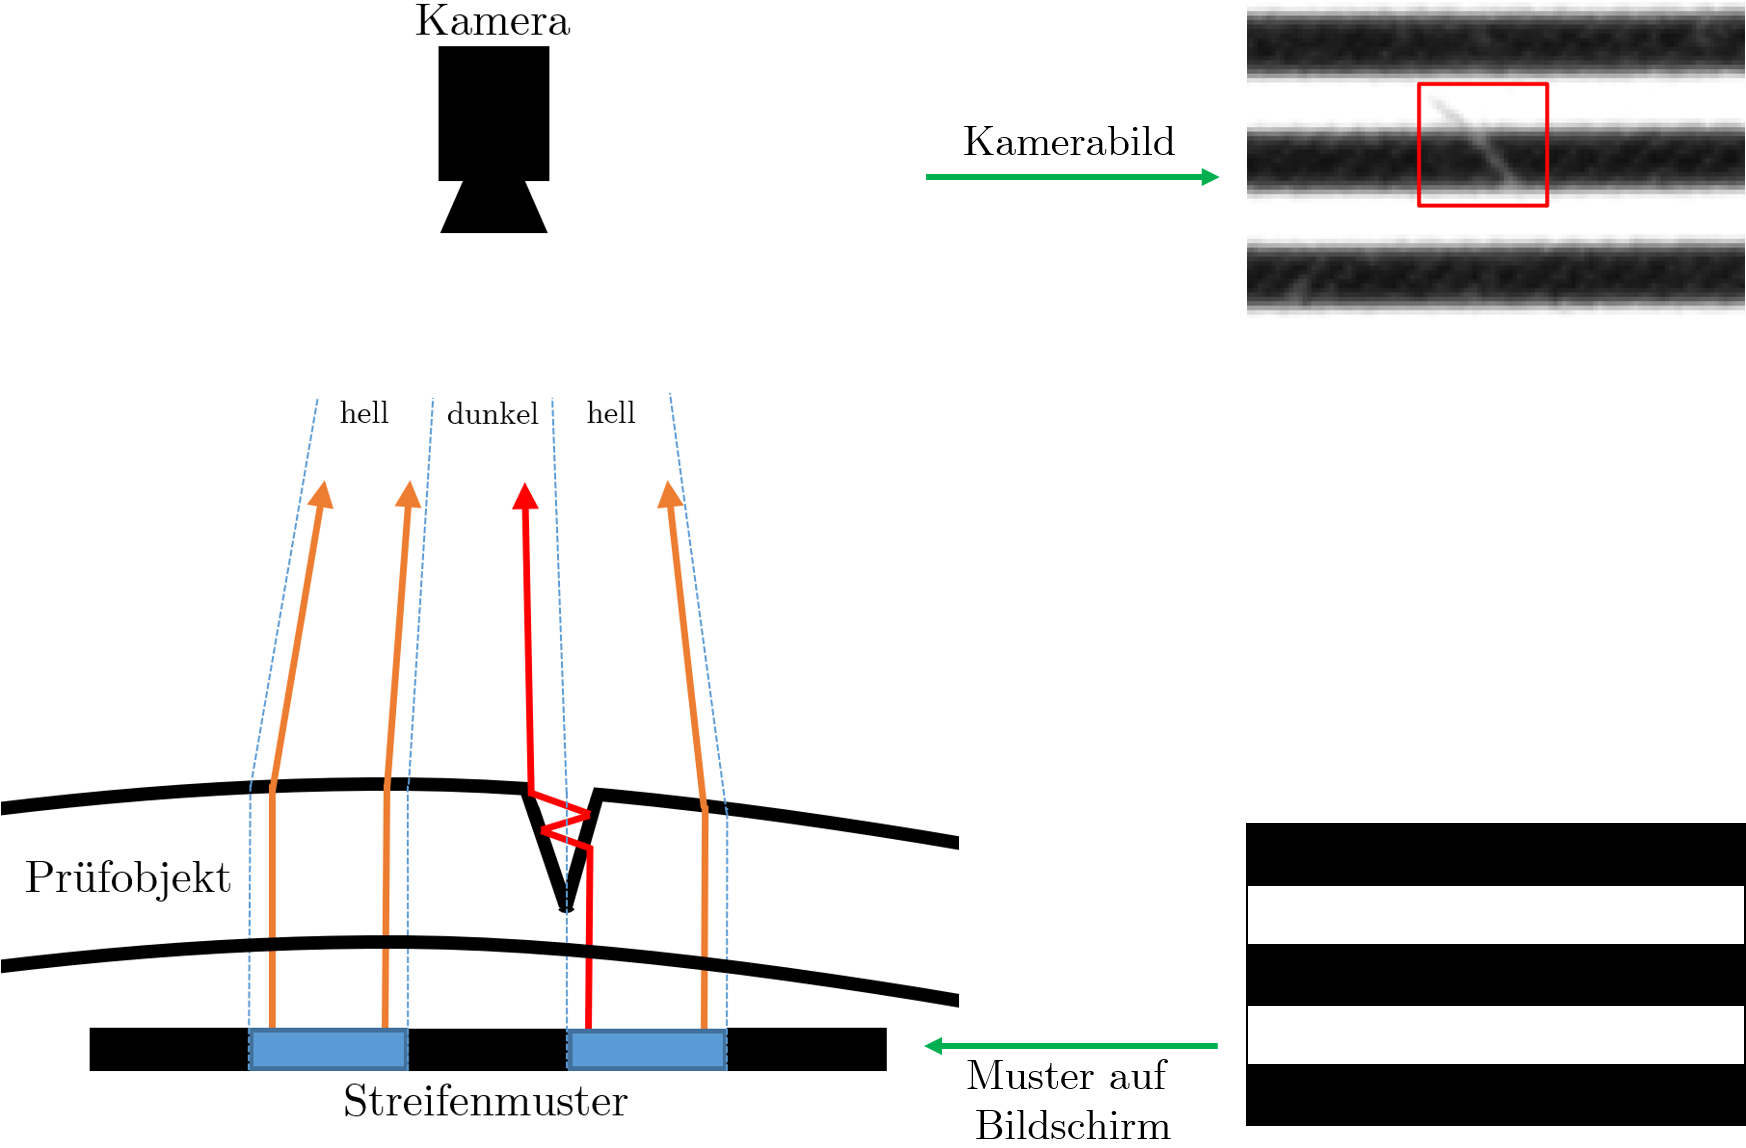
\includegraphics[width=\textwidth]{03_sichtpruefungDurchLichtstreuung/verfahren/figures/scratch_reflection_with_images}
	\caption[Lichtbrechung an einem Kratzer]{Querschnitt eines Brillenglases mit Lichtbrechung an einem Kratzer. Die blauen Stellen entsprechen den hellen Streifen und die schwarzen Stellen den dunklen Streifen auf dem Monitor. (Abbildung nicht maßstabsgetreu)}
	\label{img:lightreflection}
\end{figure}

\noindent
In Abbildung \ref{img:lightreflection} wird schematisch die Überlegung hinter dem Ansatz dargestellt.
Man nimmt ein Streifenmuster und projiziert dieses auf ein spiegelndes Prüfobjekt.
Für ein transparentes Prüfobjekt kann man das Streifenmuster als Durchlichtbeleuchtung von unten projizieren.
Mit der Kamera wird schließlich eben dieses projizierte Muster aufgenommen.
Dabei fällt an den Hell-Dunkelübergängen Licht vom hellen Streifen in den Kratzer.
Durch den Kratzer werden manche Lichtstrahlen so gestreut, dass diese an der Stelle des dunklen Streifens in den Kamerasensor gelangen (siehe roten Lichtstrahl in Abbildung \ref{img:lightreflection}).
Man erkennt im Kamerabild eine lokale Fehlstelle, da der Kratzer heller ist als der umliegende dunkle Streifen.
Analog dazu erkennt man im hellen Streifen lokal eine etwas dunklere Stelle.
Durch Anpassung der Kameraeinstellungen kann man beeinflussen, wie deutlich man den Kratzer sieht.
Z. B. kann dies durch die Erhöhung der Belichtungszeit oder weitere Öffnung der Blende geschehen.
Dadurch wird ein Oberflächendefekt im dunklen Streifen zwar besser und stärker sichtbar, allerdings ist es möglich, die Informationen über den Defekt im hellen Streifen zu verlieren.
Dies liegt daran, dass auch die dunklere Stelle im hellen Streifen so hell werden kann, dass sie nicht mehr von dem hellen Streifen selbst zu unterscheiden ist.
Dieses Problem erkennt man in der Abbildung \ref{img:scratches}.

\begin{figure}[H]
	\centering
	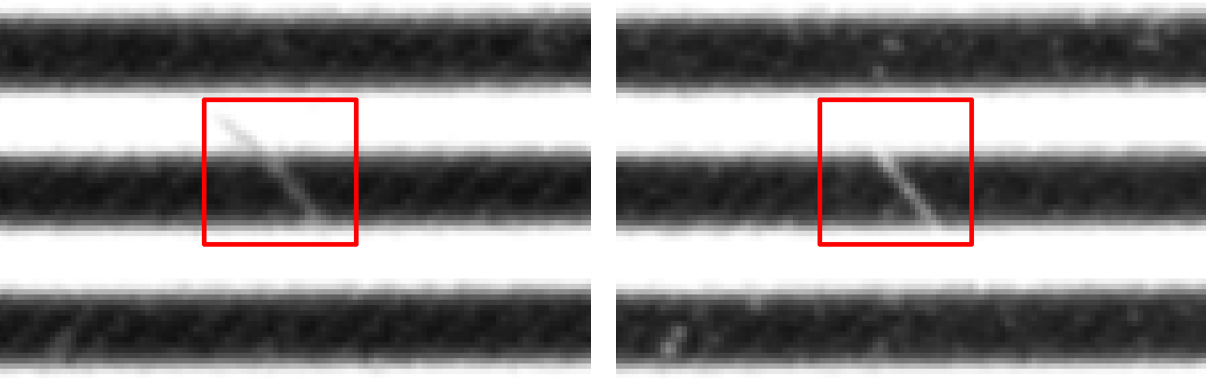
\includegraphics[width=\textwidth]{03_sichtpruefungDurchLichtstreuung/verfahren/figures/visibleScratch}
	\caption[Kratzer]{Kratzer an Hell-Dunkel-Übergang. Links mit weniger weit geöffneten Blende im Vergleich zu rechts.}
	\label{img:scratches}
\end{figure}

\noindent
Trotz der fehlenden Information hat das rechte Bild den Vorteil, dass durch den höheren Kontrast zwischen dem Oberflächendefekt und dem Hintergrund eine bessere Erkennung möglich ist.
Je ausgeprägter die Beschädigung in der Oberfläche ist, desto mehr Licht wird an der Stelle gestreut und die Beschädigung wird besser erkennbar.

\begin{figure}[H]
	\centering
	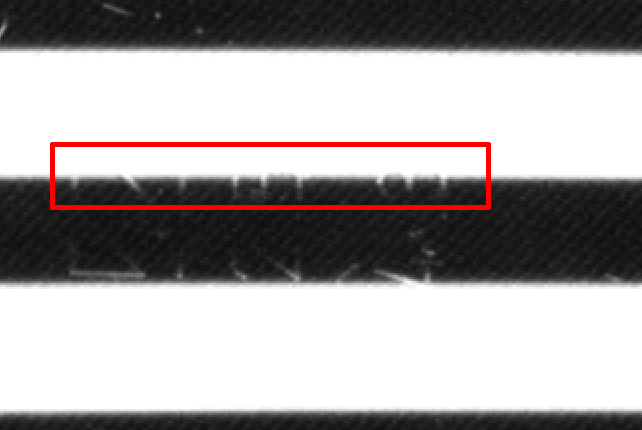
\includegraphics[width=\textwidth]{03_sichtpruefungDurchLichtstreuung/verfahren/figures/minorScratch}
	\caption[Eingravierung im Glas]{Schlecht erkennbare Eingravierung im Glas, nach Verschiebung des Streifenmusters.}
	\label{img:engraving}
\end{figure}

\noindent
In Abbildung \ref{img:engraving} stellt man fest, dass kleine Defekte der Oberflächenstruktur, wie hier z. B. die Eingravierung, nur zum Teil und besonders in der Nähe der Übergänge zu erkennen sind.

\p
Daraus lassen sich bestimmte Folgerungen ziehen.
Zunächst decken solche Streifenmuster nur unmittelbar an den Übergängen zuverlässig Defekte auf.
Das bedeutet, um Defekte an bestimmten Stellen zu erfassen, muss das verwendete Streifenmuster an den Stellen Übergänge haben.
Das bedeutet auch, dass Muster mit schmaleren Streifen aufgrund weiterer Übergänge besser geeignet sind, um auch kleinere Oberflächendefekte sichtbar zu machen.
Allerdings führt dies auch dazu, dass stets nur kleine Teile der Defekte zu erkennen sind.
Als Lösung dieses Problems kann man mehrere Streifenmuster verwenden, deren Streifen stets in ihrer Ausbreitungsrichtung verschoben sind.
Verknüpft man die sichtbaren Teile der Defekte, kann man in einem vollständigen Gesamtbild alle Oberflächendefekte ab einer bestimmten Mindeststärke sichtbar machen.
Die Mindeststärke hängt dabei unter anderem von den Kameraeinstellungen, der Beleuchtungsstärke und den verwendeten Streifenmustern ab.